\documentclass[a4paper,12pt]{article}
\usepackage[T2A]{fontenc}  %поддержка кириллицы в ЛаТеХ
\addtolength{\hoffset}{-1.7mm} % горизонтальное смещение всего текста как целого
\usepackage[utf8]{inputenc}  %По умолчанию кодировка KOI8 для *nix-систем
\usepackage[english,russian]{babel} %определение языков в документе
\usepackage{amssymb,amsmath,amsfonts,latexsym,mathtext} %расширенные наборы
  % математических символов
\usepackage{cite}  %"умные" библиографические ссылки
%(сортировка и сжатие)
\usepackage{indentfirst} %делать отступ в начале параграфа
\usepackage{enumerate}  %создание и автоматическая нумерация списков
\usepackage{tabularx}  %продвинутые таблицы
%\usepackage{showkeys}  %раскомментируйте, чтобы в документе были видны
%ссылки на литературу, рисунки и таблицы
\usepackage[labelsep=period]{caption} %заменить умолчальное разделение ':' на '.'
% в подписях к рисункам и таблицам
%\usepackage[onehalfspacing]{setspace} %"умное" расстояние между строк - установить
% 1.5 интервала от нормального, эквивалентно
 \renewcommand{\baselinestretch}{1.24}
\usepackage{graphicx} %разрешить включение PostScript-графики
\graphicspath{{Images/}} %относительный путь к каталогу с рисунками,это может быть мягкая ссылка
\usepackage{listings}

\RequirePackage{caption}
\DeclareCaptionLabelSeparator{defffis}{ -- }
\captionsetup{justification=centering,labelsep=defffis}

\usepackage{geometry} %способ ручной установки полей
\geometry{top=2cm} %поле сверху
\geometry{bottom=2cm} %поле снизу
\geometry{left=2cm} %поле справа
\geometry{right=1cm} %поле слева

\RequirePackage{totcount}
\regtotcounter{section}
\regtotcounter{page}

\usepackage[colorlinks,linkcolor=blue]{hyperref}%гиперссылки в тексте
\newcommand{\tocsecindent}{\hspace{7mm}}% отступ для введения

\makeatletter
\bibliographystyle{unsrt} %Стиль библиографических ссылок БибТеХа - нумеровать
%в порядке упоминания в тексте
\renewcommand{\@biblabel}[1]{#1.}
\makeatother

\begin{document}

%Титулный лист
\begin{titlepage}
\newpage

\begin{center}
{\small\bfМИНИСТЕРСТВО ОБРАЗОВАНИЯ И НАУКИ РОССИЙСКОЙ ФЕДЕРАЦИИ\\
ОБНИНСКИЙ ИНСТИТУТ АТОМНОЙ ЭНЕРГЕТИКИ --- филиал}\\
федерального государственного автономного образовательного учреждения\\
высшего профессионального образования\\
{\bf<<Национальный исследовательский ядерный университет <<МИФИ>>\\
(ИАТЭ НИЯУ МИФИ)}\\
\vspace{2em}
Факультет кибернетики\\
Кафедра автоматизированных систем управления
\end{center}
\vspace{2em}
УДК 004.428.4
\hfill
\parbox{5.5cm}
{
ДОПУЩЕНА К ЗАЩИТЕ\\
Заведующий кафедрой АСУ\\
д.т.н., профессор\\
\hbox to 5.5cm{\dotfill А.Н. Анохин}
}
\vspace{5em}
\begin{center}
\textbf{ВЫПУСКНАЯ РАБОТА}
\end{center}

%\vspace{2em}

\begin{center}
ИССЛЕДОВАНИЕ ГРАФИЧЕСКОГО ДВИЖКА OPTIX
\end{center}

\vspace{6em}

\hbox to \textwidth
{\parbox{6 cm}{Студент гр. ИНФ-Б10}\dotfill \parbox{4 cm}{
\begin{flushright}Еличева~Е.А.\end{flushright}}}
\vspace{2em}

\hbox to \textwidth
{\parbox{6 cm}{Руководитель\\инженер НИС ИАТЭ НИЯУ МИФИ}\dotfill \parbox{4 cm}{
\begin{flushright}Белявцев~И.П.\end{flushright}}}
\vspace{2em}

\hbox to \textwidth
{\parbox{6 cm}{Рецензент\\ научный сотрудник О-ЦОД, \\
ФГБУ <<ВНИИГМИ-МЦД>>}\dotfill \parbox{4 cm}{
\begin{flushright}Кобелев~А.Е.\end{flushright}}}

\vspace{\fill}

\begin{center}
Обнинск 2014
\end{center}

\end{titlepage}


\setcounter{page}{2} % начать нумерацию с номера три
\renewcommand{\figurename}{Рисунок}

%Меняем название Оглавления
\renewcommand{\contentsname}{\centering Содержание}
%Оглавление
\tableofcontents 
\newpage


%Введение
\begin{center}
\section*{Введение}
\addcontentsline{toc}{section}{\tocsecindent{Введение}}
\end{center}

Трассировка лучей (англ. Ray tracing; рейтрейсинг) --- один из методов геометрической оптики --- исследование оптических систем путём отслеживания взаимодействия отдельных лучей с поверхностями. В узком смысле --- технология построения изображения трёхмерных моделей в компьютерных программах, при которых отслеживается обратная траектория распространения луча (от экрана к источнику).
Данный метод имеет следующие достоинства:
\begin{enumerate}
\item возможность рендеринга гладких объектов без аппроксимации их полигональными поверхностями (например, треугольниками);
\item вычислительная сложность метода слабо зависит от сложности сцены;
\item высокая алгоритмическая распараллеливаемость вычислений — можно параллельно и независимо трассировать два и более лучей, разделять участки (зоны экрана) для трассирования на разных узлах кластера и т.д;
\item отсечение невидимых поверхностей, перспектива и корректное изменения поля зрения являются логическим следствием алгоритма.
\end{enumerate}
Серьёзным недостатком метода обратного трассирования является производительность. 
Метод растеризации и сканирования строк использует когерентность данных, чтобы распределить вычисления между пикселями. 
В то время как метод трассирования лучей каждый раз начинает процесс определения цвета пикселя заново, рассматривая каждый луч наблюдения в отдельности. 
Впрочем, это разделение влечёт появление некоторых других преимуществ, таких как возможность трассировать больше лучей, чем предполагалось для устранения контурных неровностей в определённых местах модели. 
Также это регулирует отражение лучей и эффекты преломления, и в целом — степень фотореалистичности изображения.\cite{Wiki}

Для трассировки лучей NVIDIA предлагает программную библиотеку Optix, позволяющую разработчикам программного обеспечения быстро создавать приложения на основе трассировки лучей и быстро достигать результатов благодаря графическим процессорам NVIDIA и традиционным программам на языке С. 
В отличие от рендерера с неизменяемым внешним видом, ограниченного определенными структурами данных или поддерживаемым языком программирования, движок OptiX носит чрезвычайно общий характер, позволяя разработчикам программного обеспечения быстро ускорять выполнение любых задач на основе трассировки лучей и выполнять их на широко доступном оборудовании.

Целью данной учебно--исследовательской работы является создание демонстрационного приложениея использованием графического движка OptiX.

Задачи, решаемые в ходе работы:
\begin{enumerate}
\item Изучение  программно-аппаратной архитектуры CUDA
\item Изучение принципов функционирования графического движка OptiX
\item Изучение процедуры установки графического движка OptiX
\item Изучение встроенных примеров графического движка OptiX
\item Разработка демонстрационного приложения
\item Выяснение перспектив применимости графического движка в прикладных приложениях
\end{enumerate}


% Глава 1. разработка обобщенной  модели процесса ППР реактора класса БН
\section{Изучение  программно-аппаратной архитектуры CUDA}
\subsection{GPGPU}
CUDA (Compute Unified Device Architecture) -- это технология от компании NVidia, предназначенная для разработки приложений для массивно-параллельных вычислительных устройств (в первую очередь для GPU начиная с серии G80).

Основными плюсами CUDA являются ее бесплатность (SDK для всех основных платформ свободно скачивается с developer.nvidia.com), простота (программирование ведется на "расширенном С") и гибкость.

Фактически CUDA является дальнейшим развитием GPGPU (General Purpose computation on GPU). Дело в том, что уже с самого начала GPU активно использовали параллельность (как вершины, так и отдельные фрагменты могут обрабатываться параллельно и независимо друг от друга, т.е. очень хорошо ложатся на параллельную архитектуру).

По мере развития GPU росла как степень распараллеливания, так и гибкость самих GPU. Самые первые GPU для PC (Voodoo) фактически представляли собой просто растеризатор с возможностью наложения текстуры и буфером глубины. Довольно быстро появились GPU с T\&L, т.е. полной обработкой вершин на самом GPU - на вход поступают трехмерные данные и на выходе получаем готовое изображение (например, Riva TNT). Однако гибкость в них была небольшой - ведь все вычисления велись в рамках фиксированного конвейера (FFP).

Следующим шагом (GeForce 2) стало появления вершинных шейдеров (расширение ARB\_ver\-tex\_prog\-ram) - обработку вершин стало возможным задавать в виде программы, написанной на специальном ассемблере. При этом вершины обрабатывались параллельно и независимо друг от друга. Ниже приводится пример простой программы на таком ассемблере.
\begin{verbatim}
!!ARBvp1.0
ATTRIB pos     = vertex.position;
PARAM  mat [4] = { state.matrix.mvp };

# transform by concatenation of modelview and projection matrices

DP4 result.position.x, mat [0], pos;
DP4 result.position.y, mat [1], pos;
DP4 result.position.z, mat [2], pos;
DP4 result.position.w, mat [3], pos;

# copy primary color
 
MOV result.color, vertex.color;
END
\end{verbatim}

Вполне логичным следующим шагом стало появление фрагментных программ (расширение ARB\_fragment\_program), позволяющим задавать расчет каждого пиксела также при помощи программы, на ассемблере. Важным моментом является то, что все эти вычисления (как для вершин, так и для фрагментов) ведутся с использованием 32-битовых floating-point чисел.

В архитектуре GPU появились отдельные вершинные и фрагментные процессоры, выполняющие соответствующие программы. Данные процессоры вначале были крайне просты - можно было выполнять лишь простейшие операции, практически полностью отсутствовало ветвление и все процессоры одного типа одновременно выполняли одну и ту же команду (классическая SIMD-архитектура).

За счет большого числа вершинных и фрагментных процессоров, выполняющих такие программы, оказалось, что по быстродействию (измеряемому в количестве floating-point операций в секунду) GPU в разы обгоняют CPU.

Заключительным шагом, превратившим GPU в мощные параллельные вычислители, стало поддержка floating-point текстур, т.е. стало возможным хранить значения в текстурах как 32-битовые floating-point числа.

В результате GPU фактически стало устройством, реализующим потоковую вычислительную модель (stream computing model) - есть потоки входных и выходных данных, состоящие из одинаковых элементов, которые могут быть обработаны независимо друг от друга. Обработка элементов осуществляется ядром (kernel) (см. рис.~\ref{gpu-programming-1}).
\begin{figure}[h]
\center{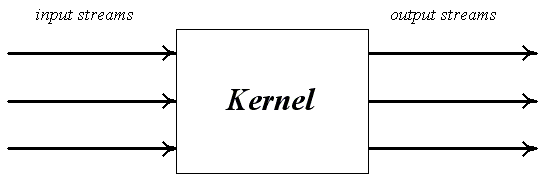
\includegraphics{gpu-programming-1.png}}
\caption{\small{Потоковые вычисления}}
\label{gpu-programming-1}
\end{figure}

Фактически GPU оказалось мощным SIMD (Single Instruction Multiple Data) процессором. В результате появилось GPGPU - использование огромной вычислительной мощности GPU для решения неграфических задач. Несмотря на значительные результаты GPGPU обладало рядом недостатков:
\begin{itemize}
\item Вся работа шла через графический API, код для GPU писался на GLSL/HLSL/Cg, остальной код - на традиционном языке программирования
\item Наличие ограничений на размеры и размерность текстур.
\item Полностью отсутствовала возможность взаимодействия между параллельно обрабатываемыми пикселами.
\item Птсутствовала поддержка так называемого scatter'а (хотя были найдены обходные пути).
\end{itemize}

Кроме того на GPU GeForce 6xxx/7xxx отсутствовала нативная поддержка целых чисел и побитовых операций над ними.

Появление CUDA (а также GPU G80) полностью сняло все эти ограничения, предложив для GPGPU простую и удобную модель. В этой модели GPU рассматривается как специализированное вычислительное устройство (называемое device), которое:
\begin{itemize}
\item Является сопроцессором к CPU (называемому host).
\item Обладает собственной памятью (DRAM).
\item Обладает возможностью параллельного выполнения огромного количества отдельных нитей (threads).
\end{itemize}

При этом между нитями на CPU и нитями на GPU есть принципиальные различия ---
\begin{itemize}
\item Нити на GPU обладают крайне "небольшой стоимостью" - их создание и управление требует минимальных ресурсов (в отличии от CPU).
\item Для эффективной утилизации возможностей GPU нужно использовать многие тысячи отдельных нитей (для CPU обычно нужно не более 10-20 нитей).
\end{itemize}

Сами программы пишутся на "расширенном" С, при этом их параллельная часть (ядра) выполняется на GPU, а обычная часть - на CPU. CUDA автоматически осуществляет разделением частей и управлением их запуском.

CUDA использует большое число отдельных нитей для вычислений, часто каждому вычисляемому элементами соответствует одна нить. Все нити группируются в иерархию - grid/block/thread (см. рис.~\ref{cuda-1}).
\begin{figure}[h]
\center{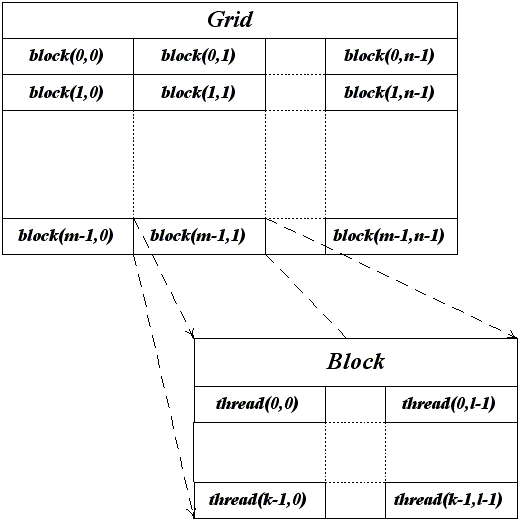
\includegraphics{cuda-1.png}}
\caption{\small{Иерархия нитей в CUDA}}
\label{cuda-1}
\end{figure}

Верхний уровень - grid - соответствует ядру и объединяет все нити выполняющие данное ядро. grid представляет собой одномерный или двухмерный массив блоков (block). Каждый блок (block) представляет из себя одно/двух/трехмерный массив нитей (threads).

При этом каждый блок представляет собой полностью независимый набор взаимодействующих между собой нитей, нити из разных блоков не могут между собой взаимодействовать.

Фактически блок соответствует независимо решаемой подзадаче, так например если нужно найти произведение двух матриц, то матрицу-результат можно разбить на отдельные подматрицы одинакового размера. Нахождение каждой такой подматрицы может происходить абсолютно независимо от нахождения остальных подматриц. Нахождение такой подматрицы - задача отдельного блока, внутри блока каждому элементу подматрицы соответствует отдельная нить.

При этом нити внутри блока могут взаимодействовать между собой (т.е. совместно решать подзадачу) через
\begin{itemize}
\item Общую память (shared memory).
\item Функцию синхронизации всех нитей блока (\_\_synchronize).
\end{itemize}

Подобная иерархия довольно естественна - с одной стороны хочется иметь возможность взаимодействия между отдельными нитями, а с другой - чем больше таких нитей, тем выше оказывается цена подобного взаимодействия.

Поэтому исходная задача (применение ядра к входным данным) разбивается на ряд подзадач, каждая из которых решается абсолютно независимо (т.е. никакого взаимодействия между подзадачами нет) и в произвольном порядке.

Сама же подзадача решается при помощи набора взаимодействующих между собой нитей.

С аппаратной точки зрения все нити разбиваются на так называемые warp'ы --- блоки подряд идущих нитей, которые одновременно (физически) выполняются и могут взаимодействовать друг с другом. Каждый блок нитей разбивается на несколько warp'ов, размер warp'а для всех существующих сейчас GPU равен 32.

Важным моментом является то, что нити фактически выполняют одну и ту же команды, но каждая со своими данными. Поэтому если внутри warp'а происходит ветвление (например в результате выполнения оператора if), то все нити warp'а выполняют все возникающие при этом ветви. Поэтому крайне желательно уменьшить ветвление в пределах каждого отдельного warp'а.

Также используется понятие half-warp'а --- это первая или вторая половина warp'а. Подобное разбиение warp'а на половины связано с тем, что обычно обращение к памяти делаются отдельно для каждого half-warp'а.

Кроме иерархии нитей существует также несколько различных типов памяти. Быстродействие приложения очень сильно зависит от скорости работы с памятью. Именно поэтому в традиционных CPU большую часть кристалла занимают различные кэши, предназначенные для ускорения работы с памятью (в то время как для GPU основную часть кристалла занимают ALU).

В CUDA для GPU существует несколько различных типов памяти, доступных нитям, сильно различающихся между собой (см. табл.~\ref{cudatypes}).

\begin{table}[h]
\caption{\label{cudatypes}\small{ Типы памяти в CUDA.}}
\begin{center}
\begin{tabular}{|l|l|l|l|}
\hline
Тип памяти	&Доступ	&Уровень выделения 	&Скорость работы \\
\hline
регистры (registers)	&R/W	&per-thread	&высокая (on chip)\\
\hline
local	&R/W	&per-thread	&низкая (DRAM)\\
\hline
shared	&R/W	&per-block	 &высокая (on-chip)\\
\hline
global	&R/W	&per-grid	&низкая(DRAM)\\
\hline
constant	&R/O 	&per-grid	&высокая(on chip L1 cache)\\
\hline
texture	&R/O	 &per-grid	&высокая(on chip L1 cache)\\
\hline
\end{tabular}
\end{center}
\end{table} 
При этом CPU имеет R/W доступ только к глобальной, константной и текстурной памяти (находящейся в DRAM GPU) и только через функции копирования памяти между CPU и GPU (предоставляемые CUDA API).

\subsection{Расширения языка С}

Программы для CUDA (соответствующие файлы обычно имеют расширение .cu) пишутся на "расширенном" С и компилируются при помощи команды nvcc.

Вводимые в CUDA расширения языка С состоят из:
\begin{itemize}
\item Спецификаторов функций, показывающих где будет выполняться функция и откуда она может быть вызвана.
\item Спецификаторы переменных, задающие тип памяти, используемый для данной переменных.
\item Директива, служащая для запуска ядра, задающая как данные, так и иерархию нитей.
\item Встроенные переменные, содержащие информацию о текущей нити.
\item runtime, включающий в себя дополнительные типы данных.
\end{itemize}

\subsubsection{Спецификаторы}

\begin{table}[h]
\caption{\label{cudatypes} \small{Спецификаторы функций в CUDA.}}
\begin{center}
\begin{tabular}{|l|l|l|}
\hline
Спецификатор	&Выполняется на	&Может вызываться из \\
\hline
\_\_device\_\_	&device	&device\\
\hline
\_\_global\_\_	&device	&host\\
\hline
\_\_hos\_\_	&host	&host\\
\hline
\end{tabular}
\end{center}
\end{table} 

При этом спецификаторы\_\_host\_\_ и \_\_device\_\_ могут быть использованы вместе (это значит, что соответствующая функция может выполняться как на GPU, так и на CPU --- соответствующий код для обеих платформ будет автоматически сгенерирован компилятором). Спецификаторы \_\_global\_\_ и \_\_host\_\_ не могут быть использованы вместе.

Спецификатор \_\_global\_\_ обозначает ядро и соответствующая функция должна возвращать значение типа void.

\begin{verbatim}
__global__ void myKernel ( float * a, float * b, float * c )
{
    int index = threadIdx.x;
	
    c [i] = a [i] * b [i];
}
\end{verbatim}

На функции, выполняемые на GPU (\_\_device\_\_ и \_\_global\_\_) накладываются следующие ограничения:
\begin{itemize}
\item Нельзя брать их адрес (за исключением \_\_global\_\_ функций).
\item Не поддерживается рекурсия.
\item Не поддерживаются static-переменные внутри функции.
\item Не поддерживается переменное число входных аргументов.
\end{itemize}

Для задания размещения в памяти GPU переменных используются следующие спецификаторы --- \_\_device\_\_, \_\_constant\_\_ и \_\_shared\_\_. На их использование также накладывается ряд ограничений:
\begin{itemize}
\item Эти спецификаторы не могут быть применены к полям структуры (struct или union).
\item Соответствующие переменные могут использоваться только в пределах одного файла, их нельзя объявлять как extern.
\item Запись в переменные типа \_\_constant\_\_ может осуществляться только CPU при помощи специальных функций.
\item \_\_shared\_\_ переменные не могут инициализироваться при объявлении.
\end{itemize}

\subsubsection{Добавленные переменные}

В язык добавляются 1/2/3/4--мерные вектора из базовых типов -- char1, char2, char3, char4, uchar1, uchar2, uchar3, uchar4, short1, short2, short3, short4, ushort1, ushort2, ushort3, ushort4, int1, int2, int3, int4, uint1, uint2, uint3, uint4, long1, long2, long3, long4, ulong1, ulong2, ulong3, ulong4, float1, float2, float3, float2, и double2.

Обращение к компонентам вектора идет по именам --- x, y, z и w. Для создания значений --- векторов заданного типа служит конструкция вида make\_<typeName>.

\begin{verbatim}
int2   a = make_int2   ( 1, 7 );
float3 u = make_float3 ( 1, 2, 3.4f );
\end{verbatim}

Обратите внимание, что для этих типов (в отличии от шейдерных языков GLSL/Cg/HLSL) не поддерживаются векторные покомпонентные операции, т.е. нельзя просто сложить два вектора при помощи оператора "+" --- это необходимо явно делать для каждой компоненты.

Также для задания размерности служит тип dim3, основанный на типе uint3, но обладающий нормальным конструктором, инициализирующим все не заданные компоненты единицами.

\subsubsection{Директива вызова ядра}

Для запуска ядра на GPU используется следующая конструкция:
\begin{verbatim}
kernelName <<<Dg,Db,Ns,S>>> ( args )
\end{verbatim}
Здесь kernelName это имя (адрес) соответствующей \_\_global\_\_ функции, Dg --- переменная (или значение) типа dim3, задающая размерность и размер grid'a (в блоках), Db --- переменная (или значение) типа dim3, задающая размерность и размер блока (в нитях), Ns --- переменная (или значение) типа size\_t, задающая дополнительный объем shared--памяти, которая должна быть динамически выделена (к уже статически выделенной shared-памяти), S -- переменная (или значение) типа cudaStream\_t задает поток (CUDA stream), в котором должен произойти вызов, по умолчанию используется поток 0. Через args обозначены аргументы вызова функции kernelName.

Также в язык С добавлена функция \_\_syncthreads, осуществляющая синхронизацию всех нитей блока. Управление из нее будет возвращено только тогда, когда все нити данного блока вызовут эту функцию. Т.е. когда весь код, идущий перед этим вызовом, уже выполнен (и, значит, на его результаты можно смело рассчитывать). Эта функция очень удобная для организации безконфликтной работы с shared-памятью.

Также CUDA поддерживает все математические функции из стандартной библиотеки С, однако с точки зрения быстродействия лучше использовать их float--аналоги (а не double) --- например sinf. Кроме этого CUDA предоставляет дополнительный набор математических функций (\_\_sinf, \_\_powf и т.д.) обеспечивающие более низкую точность, но заметно более высокое быстродействие чем sinf, powf и т.п. \cite{cudawiki}

% Глава 2. Алгоритмы для расчета порядка процесса ППР реактора класса БН
%\input{Graph}

%\input{Development}

%\input{Outro}

%Список литературы
%Библиография
\newpage
\addcontentsline{toc}{section}{\tocsecindent{Список литературы}}
\begin{thebibliography}{0}
\bibitem{Ukr}
С.А.~Андрушечко, А.М.~Арфов, Б.Ю.~Васильев, В.Н.~Генералов, К.Б.~Косоуров, Ю.М.~Семченков, В.Ф.~Украинцев. АЭС с реактором типа ВВЭР-1000. От физических основ эксплуатации до эволюции проекта. --- 
М.: Логос, 2010. --- 604 с.: ил.
ISBN 978-5-98704-496-4

\bibitem{BH}
Г.Б.~Усынин, Е.В.~Кусмарцев. Реакторы на быстрых нейтронах: Учеб. пособие для вузов/Под ред. Ф.М.~Митенкова. --- 
М.: Энергоатомиздат, 1985. --- 288 с.: ил.

\bibitem{NIIAR}
Официальный сайт ОАО ``ННЦ НИИАР'' (\href{http://www.niiar.ru/}{www.niiar.ru})

\bibitem{TA}
Джон Хопкрофт, Раджив Мотвани, Джеффри Ульман Введение в теорию автоматов, языков и вычислений = Introduction to Automata Theory, Languages, and Computation. --- 
М.: Вильямс, 2002. --- 528 c. 
ISBN 0-201-44124-1

\bibitem{Nosov}
В.И.~Носов, Т.В.~Бернштейн, Н.В.~Носкова, Т.В.~Храмова. Элементы теории графов. Учебное пособие. ---
Новосибирск, 2008. --- 107 с.

\bibitem{AI}
С.Дж.~Рассел, П.~Норвиг. Искусственный интеллект: современный подход = Artificial Intelligence: A Modern Approach / Пер. с англ. и ред. К. А. Птицына. --- 2-е изд.. --- 
М.: Вильямс, 2006. --- 157—162 cc.
ISBN 5-8459-0887-6

\bibitem{habr}
Д.~Восквитцов. Реализация графов и деревьев на Python

\bibitem{PyGraph}
Гвидо ван Россум, Шаблоны Python --- реализация графов = Python Patterns - Implementing Graphs / Пер. с англ. С.Тезадов. 

\bibitem{networkX}
Официальный сайт проекта NetworkX (\href{http://networkx.lanl.gov/reference/index.html}{http://networkx.lanl.gov/reference/index.html})
\end{thebibliography}




\end{document}   